\documentclass[a4paper]{article}
\usepackage[UTF8]{ctex}
\usepackage{geometry}
\usepackage{graphicx}
\usepackage{url}
\usepackage{multirow}
\usepackage{array}
\usepackage{booktabs}
\usepackage{url}
\usepackage{enumitem}
\usepackage{graphicx}
\usepackage{float}
\usepackage{amssymb}
\usepackage{amsmath}
\usepackage{subfig}
\usepackage{longtable}
\usepackage{pifont}
\usepackage{color}

\allowdisplaybreaks

\geometry{a4paper, scale=0.78}

\usepackage{tikz}
\newcommand*{\circled}[1]{\lower.7ex\hbox{\tikz\draw (0pt, 0pt)%
    circle (.5em) node {\makebox[1em][c]{\small #1}};}}
    

% \begin{figure}[H]
%     \centering
%     \includegraphics[width=.55\textwidth]{E.png}
%     \caption{矩阵与列向量的乘法}
%     \label{fig:my_label_1}
% \end{figure}

% \left\{
% \begin{array}{ll}
%       x+2x+z=2 & \\
%       3x+8y+z=12 & \\
%       4y+z=2
% \end{array}
% \right.

% \begin{enumerate}[itemindent = 1em, itemsep = 0.4pt, parsep=0.5pt, topsep = 0.5pt]

% \end{enumerate}

%\stackrel{a}{\longrightarrow}

%\underbrace{}_{} %下括号

%\tableofcontents %目录,并且目录页不记录页码
% \tableofcontents
% \newpage
% \setcounter{page}{1} %new page
% \clearpage

\title{Boltzmann Machine}
\author{Chen Gong}
\date{08 April 2020}

\begin{document}
\maketitle
%\pagestyle{empty}
\tableofcontents
\newpage
%\pagestyle{fancy}
\setcounter{page}{1} %new page
\clearpage

玻尔兹曼机(Boltzmann Machine)在“受限玻尔兹曼机”那一章就有了简单的描述。在那一章我们就较为详细的分析过了,由于Boltzmann machine中的依赖关系过于复杂,它的Learning和Inference问题基本是intractable。所以,为了简化而提出了受限玻尔兹曼机(Restricted Boltzmann Machine)。但是,为什么又重新谈谈这个似乎不太好的模型呢?主要原因是Boltzmann Machine是深度信念网络(DBN),前馈神经网络等网络结构的基础,大名鼎鼎的变分推断(Variational Inference)也是Hinton为求解Boltzmann machine而提出的。
\section{Introduction}
Boltzmann machine节点之间为任意连接,节点可以分为可观测变量$v$和不可观测变量$h$。每个节点都符合$\{0,1\}$的伯努利分布。Boltzmann machine模型的概率图示意图如下所示:
\begin{figure}[H]
    \centering
    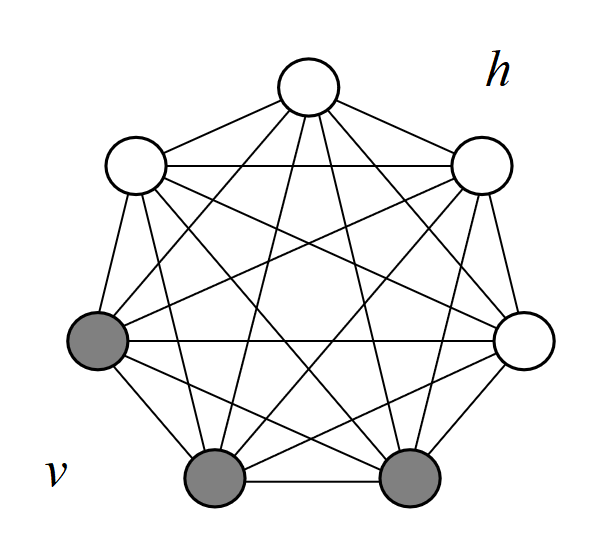
\includegraphics[width=.45\textwidth]{微信图片_20200409150446.png}
    \caption{Boltzmann machine模型的概率图}
    \label{fig:my_label_1}
\end{figure}
其中,$v_{D\times 1} \in \{0,1\}^D$,$h_{P\times 1} \in \{0,1\}^P$。根据“受限玻尔兹曼”那节的知识,可以得出,概率图的联合概率分布为:
\begin{equation}\left\{\begin{array}{l}
P(v, h)=\frac{1}{2} \exp \{-\text{E}(v, h)\} \\
\text{E}(v, h)=-\left(v^{\top} \cdot W \cdot h+\frac{1}{2} v^{\top} \cdot L v+\frac{1}{2} h^{\top} \cdot J \cdot h\right)
\end{array}\right.\end{equation}
其中,$L=[L_{ij}]_{D\times D}$,$J=[J_{ij}]_{P\times P}$,$W= [w_{ij}]_{D\times P}$。我相信坚持学到这里的同学们,对于机器学习的数学推导变换一定有了较好的基础。\textbf{实际上矩阵的相乘就是用简单的方式来表示连加,在涉及到求导运算时,矩阵相乘来代替连加符号,可以简化推导过程。}比如,$v^{\top} \cdot W \cdot h = \sum_{i=1}^D \sum_{j=1}^P v_iw_{ij}h_j$。而$\frac{1}{2} v^{\top} \cdot L v$前面为什么要乘上$1/2$呢?实际上打开就知道了,$v^{\top} \cdot L v = \sum_{i=1}^D \sum_{j=1}^D v_iw_{ij}v_j$,那么很显然$v_iw_{ij}v_j = v_jw_{ji}v_i$。所以,所有的值都被加了两次,而我们的目的只要求$v$集合中的任意两个点的乘积,只需要加一次即可,当然需要乘上$\frac{1}{2}$。

而这个$\frac{1}{2}$又乘与不乘都没有关系,因为$\frac{1}{2}$可以藏在$L$里面,在Learning的过程中,自动的缩小$\frac{1}{2}$就可以了。在此问题中,要学习的参数集合为$\theta = \{ W,L,J \}$。

\section{基于极大似然的梯度上升}
既然是基于极大似然的梯度上升,显然离不开两个部分,极大似然函数和梯度。总所周知,\textbf{极大似然估计的主要思路是,使极大似然函数最大时的参数。}首先明确一下,要求的参数为$\theta = \{ W,L,J \}$。样本集合$v$,$|v|=D$。那么,似然函数为:
$$\sum_v P(v) = \sum_v \sum_{h}P(v,h)$$
那么对数似然函数为(实际上$\frac{1}{D}$加不加对于求解没有什么关系,为了严谨起见还是加上):
$$\frac{1}{D}\sum_v \log P(v)$$
\subsection{似然导数求解}
那么,下一步就是对对数似然函数求导,即为:
\begin{equation}
\frac{\partial}{\partial \theta} \frac{1}{D} \sum_{v} \log p(v)=\frac{1}{D} \sum_{v} \frac{\partial \log p(v)}{\partial \theta}
\end{equation}
在“直面配分函数”那章的公式(27),我们已经详细的推导了Boltzmann Distribution的log似然梯度,
\begin{equation}\begin{aligned}
\frac{1}{D} \frac{\partial}{\partial \theta} \log P(v) 
&=\frac{1}{D}\left(\sum_{h} \sum_{v} P(h, v) \frac{\partial}{\partial \theta} \mathrm{E}(h, v)-\sum_{h} P(h | v) \frac{\partial}{\partial \theta} \mathrm{E}(h, v)\right)
\end{aligned}\end{equation}
我们主要研究的是对$w$的求导,对其他两个参数矩阵的求导都一样,而且比$w$要更简单一点,这里主要是对$w$求导。小编狠下心来,系统的看了一下矩阵求导,迟早都要学的,建议大家也可以系统的看看,挺有帮助的。那么对$w$参数矩阵的求导如下所示:
\begin{equation}\begin{aligned}
\frac{\partial \log p(v)}{\partial W} &=\sum_{v} \sum_{h} p(v, h) \cdot-\left(v h^{\top}\right) - \sum_{h} p(h | v) \cdot - \left(v h^{\top}\right) \\
&=\sum_{i} p(h | v) \cdot v h^{\top}-\sum_{\top} \sum_{h} p(v, h) \cdot v h^{\top}
\end{aligned}\end{equation}
其中,$\text{E}(v, h)=-\left(v^{\top}Wh+\frac{1}{2} v^{\top} L v+\frac{1}{2} h^{\top} J h\right)$。注意一下,这里的$v$和$h$矩阵的大小分别为,$D\times  1$和$P\times 1$。$v^{\top}Wh$是一个一维的,那么对$W_{D\times  P}$求导,得到的也必然是一个$D\times  P$的矩阵。那么,很简单可以得到:
\begin{equation}
\frac{1}{D} \sum_{v} \frac{\partial \log P(v)}{\partial W}=\frac{1}{D} \sum_{v} \sum_{h} p(h | v) \cdot v h^{T}-\frac{1}{D} \sum_{v} \sum_{v} \sum_{h} P(v, h)\cdot v h^{T}
\end{equation}
看到其中的$\frac{1}{D} \sum_{v} \sum_{v} \sum_{h} P(v, h)\cdot v h^{T}$,对$v$和$h$求完和以后,显然$\sum_{v} \sum_{h} P(v, h)\cdot v h^{T}$是一个常数$C$。所以,$frac{1}{D} \sum_{v} \sum_{v} \sum_{h} P(v, h)\cdot v h^{T} = \frac{1}{D} \sum_{v} C = \frac{1}{D} D\cdot C = \sum_{v} \sum_{h} P(v, h)\cdot v h^{T}$。所以,公式(5)可以改写为:
\begin{equation}
\frac{1}{D} \sum_{v} \frac{\partial \log P(v)}{\partial W}=\frac{1}{D} \sum_{v} \sum_{h} P(h | v) \cdot v h^{T}- \sum_{v} \sum_{h} P(v, h)\cdot v h^{T}
\end{equation}
而公式(6)可以被简写为:
\begin{equation}
\frac{1}{D} \sum_{v} \frac{\partial \log P(v)}{\partial W}=\mathbb{ E}_{P_{\text {data }}}\left[v h^{\top}\right]- \mathbb{E}_{P_{\text {model }}}\left[v h^{\top}\right]
\end{equation}
其中,
\begin{equation}
    \begin{split}
        & P_{\text{data}} =P_{\text{data}} (v) \cdot P_{\text {model }}(h | v) \\
        & P_{\text {model }}=P_{\text {model }}(v, h) 
    \end{split}
\end{equation}
为什么这样表达呢?实际上老师说的很模糊,我谈谈自己的理解。在$\sum_{v} \sum_{h} P(v, h)$中,$P(v,h)$是生成模型,本身就是我们建立的模型,所以被称为$P_{\text{model}}$。而在$\sum_{v} \sum_{h} P(h | v)$首先从经验分布$P(v)$从采样得到$v$,然后利用模型分布来求解$P(h | v)$,所以$P_{\text{data}} =P_{\text{data}} (v) \cdot P_{\text {model }}(h | v)$。采样出$ P_{\text {model }}(h | v)$和$P_{\text {model }}(v)$就可以求解出$P_{\text {model }}(h,v)$了。按照同样的方法可以求得对$\{L,J\}$的导数。
\subsection{似然梯度下降法汇总}
\begin{itemize}
    \item Boltzmann Machines中的节点可以分为可观测变量集合$v$和不可观测变量集合$h$。每个节点属于0/1分布,$v_{D\times 1} \in \{0,1\}^D$,$h_{P\times 1} \in \{0,1\}^P$。
    \item 参数集合为:$\theta = \{ W,L,J \}$。参数矩阵的大小为:$L=[L_{ij}]_{D\times D}$,$J=[J_{ij}]_{P\times P}$,$W= [w_{ij}]_{D\times P}$。
    \item Boltzmann Distribution的模型表示为:
    \begin{equation}\left\{\begin{array}{l}
    P(v, h)=\frac{1}{2} \exp \{-\text{E}(v, h)\} \\
    \text{E}(v, h)=-\left(v^{\top} \cdot W \cdot h+\frac{1}{2} v^{\top} \cdot L v+\frac{1}{2} h^{\top} \cdot J \cdot h\right)
    \end{array}\right.\end{equation}
    \item 求解参数用到极大似然估计,Log-Likelihood Function为:
    \begin{equation}
        \frac{1}{D}\sum_v \log P(v)
    \end{equation}
    \item 通过计算可以得到每个参数矩阵的似然梯度为:
    \begin{equation}\left\{\begin{array}{l}
    \Delta W=\alpha \left(\mathbb{E}_{p_{data}}\left[v h^{\top}\right]-\mathbb{E}_{p_{\text{model}}}\left[v h^{\top}\right]\right) \\
    \Delta L=\alpha \left(\mathbb{E}_{p_{data}}\left[v v^{\top}\right]-\mathbb{E}_{p_{\text{model}}}\left[v v^{\top}\right]\right) \\
    \Delta J=\alpha \left(\mathbb{E}_{p_{data}}\left[h h^{\top}\right]-\mathbb{E}_{p_{\text{model}}}\left[h h^{\top}\right]\right)
    \end{array}\right.\end{equation}
    其中:
    \begin{equation}
        \left\{
        \begin{array}{ll}
            P_{\text{data}} =P_{\text{data}} (v) \cdot P_{\text {model }}(h | v) & \\
            P_{\text {model }}=P_{\text {model }}(v, h)  & \\
        \end{array}
        \right.
    \end{equation}
\end{itemize}

\subsection{小结}
通过上述的求解发现,梯度的统计量只和$v,h$相关,只不过分布不一样而已。RBM也是一种特殊的Boltzmann Machines,RBM的求解比较的简单。在“直面配分函数”那一章中可以看到,RBM在化简完毕后,$P_{\text{data}} =P_{\text{data}} (v)$不需要考虑$P_{\text {model }}(h | v)$,这样计算起来就非常简单,梯度在理论上很干净。在前馈神经网络中Gradient需要使用链式求导法则,计算起来非常的复杂。而这里就不一样,只要解决了后验$P_{\text {model }}(h | v)$就可以了。那么,下一个重点就是如何从后验$P_{\text {model }}(h | v)$中进行采样。

\section{基于MCMC的似然梯度下降}
\subsection{MCMC似然梯度求解总述}
在第二小节中,我们已经讲到了,使用梯度上升法来使log似然函数达到最大,从而求解对应的最优参数。参数更新公式为:
\begin{equation}
    \theta^{(t+1)} = \theta^{(t)} + \triangle \theta
\end{equation}
其中,$\triangle \theta = \{ \triangle W, \triangle L, \triangle J \}$。以$\triangle W$为例,$\triangle W$是一个矩阵$\triangle W = [\triangle w_{ij}]$。其中,
\begin{equation}
    \triangle w_{ij} = \alpha \left[ \underbrace{\mathbb{E}_{P_{\text{data}}}[v_ih_j]}_{\text{Postive phase}} - \underbrace{\mathbb{E}_{P_{\text{model}}}[v_ih_j]}_{\text{Negative phase}} \right]
\end{equation}

这个Postive和Negative phase的说法,我们在“直面配分函数”那章有详细的描述。那么,\textbf{现在的难点就是$v_ih_j$从何而来。}

回忆一下,在RBM中,$P(h | v)$是可以直接求出来的。
\begin{equation}
P(h | v)=\prod_{l=1}^{m} P\left(h_{l} | v\right)=\left(\sigma\left(\sum_{j=1}^{n} w_{l j} v_{i}+\beta_{l}\right)\right)^{k}\left(1-\sigma\left(\sum_{j=1}^{n} w_{l j} v_{i}+\beta_{l}\right)\right)^{m-k}
\end{equation}
而$P_{\text{data}}$直接从样本中进行采样就可以了,而$P_{\text{model}}(v,h)$为:
\begin{equation}\begin{aligned}
P(h, v) h_{i} v_{j} &=\sum_{h} \sum_{v} P(v) P(h | v) h_{i} v_{j} \\
&=\sum_{v} P(v) \sum_{h} P(h | v) h_{i} v_{j} \\
&=\frac{1}{Z} \exp \left(\alpha^{T} v+\sum_{i=1}^{m} \log \left(1+\exp \left(w_{i} v+\beta_{i}\right)\right)\right) \sigma\left(\sum_{j=1}^{n} w_{i j} v_{i}+\beta_{i}\right) v_{j}
\end{aligned}\end{equation}
这个分布过于复杂,当时采用的是基于对于散度的Gibbs采样来解决。而在Boltzmann Machines中,Postive phase和Negative phase都是Intractable。所以,Hinton提出了用MCMC来对$P(h|v)$进行采样。

\textbf{这里再明确一下逻辑,在求解$\triangle W$中,主要是解决三个部分,$P_{\text{data}} (v),P_{\text {model }}(h | v),P_{\text {model }}(v, h)$,其中$P_{\text {model }}(v, h) = P_{\text {model }}(h | v)\cdot P_{\text {model }}(v)$。 所以,而$P_{\text{data}} (v)$和$P_{\text {model }}(v)$相对比较简单,所以难点在于$P_{\text {model }}(h | v)$的求解。而在RBM中$P_{\text {model }}(h | v)$比较容易求解,而$P_{\text {model }}(v, h)$过于复杂,所以要采用MCMC来解决。而在Boltzmann Machines中,由于关系过于复杂,没有办法分解,甚至最大团分解都没有用,因为最大团就是自己,那么连$P_{\text {model }}(h | v)$都求不出来,那么Postive phase和Negative phase都是Intractable。}

很幸运的是,通过推导,可以得到:
\begin{equation}\begin{array}{l}
P\left(v_{i}=1 | h, v_{-i}\right)=\sigma\left(\sum_{j=1}^{P} w_{i j} h_{j}+\sum_{k=1\setminus i}^{D} L_{i k} v_{k}\right) \\
P\left(h_{j}=1 | v, h_{-j}\right)=\sigma\left(\sum_{i=1}^{D} w_{i j} v_{i}+\sum_{m=1\setminus j}^{p} J_{j m} h_{n}\right)
\end{array}\end{equation}
解释一下,这两个公式是什么意思。公式表达的是,在已知一个节点以外的所有的点的条件下,这个节点的条件概率是可求的。其中$1\setminus i$表达的意思是$1 \sim D$但不包括$i$的所有节点。

为什么说很幸运呢?因为真实的后验是求不出来的,但是MCMC提供了一种一维一维的采样的方法(Gibbs采样法)。而每一个维的概率分布可以求出来,那么Gibbs采样就可以很愉快的被使用了。而且,这个结论同时也可以在RBM中使用,下面我们来举个例子,假设有一个RBM,如下图所示:
\begin{figure}[H]
    \centering
    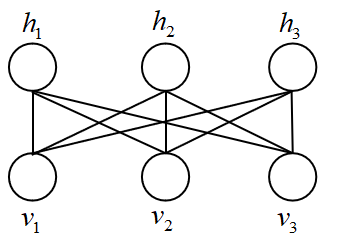
\includegraphics[width=.35\textwidth]{微信图片_20200414173610.png}
    \caption{RBM概率图模型}
    \label{fig:my_label_1}
\end{figure}
由于在已知$v$的情况下,$h$中的节点都是相互独立的,所以:
\begin{equation}P(h | v)=\prod_{j=1}^{3} p\left(h_{j} | v\right)\end{equation}
同理可得:
\begin{equation}P\left(h_{j} = 1| v\right)=P\left(h_{j} =1 | v, h_{-j}\right)=\sigma \left(\sum_{i=1}^{D} w_{ij} v_{i}+0\right)\end{equation}
为什么$\sum_{m=1\setminus j}^{p} J_{j m} h_{n} = 0$呢?因为,$h$节点内部都是相互独立的,没有边,所有都是0。实际上在RBM那一章,后验是花了较大的功夫去求的。而使用公式(17)给出的结论,我们可以较为简单的写出。可以看到,由于RBM的特殊性质,$h$集合之间相互独立,分解起来非常简单。在BM就没有这么好了,虽然每一维可以求出来,由于无法分解,求解起来根本就不可能。

\subsection{条件概率推导}
在3.1节中,给出了两个条件概率分布:
\begin{equation}\begin{array}{l}
P\left(v_{i}=1 | h, v_{-i}\right)=\sigma\left(\sum_{j=1}^{P} w_{i j} h_{j}+\sum_{k=1\setminus i}^{D} L_{i k} v_{k}\right) \\
P\left(h_{j}=1 | v, h_{-j}\right)=\sigma\left(\sum_{i=1}^{D} w_{i j} v_{i}+\sum_{m=1\setminus j}^{p} J_{j m} h_{n}\right)
\end{array}\end{equation}
这一节,就来详细的推导一下:
\begin{equation}\begin{aligned}
P\left(v_{i} | h, v_{-i}\right)&=\frac{P(v, h)}{P(h, v_{-i})}=\frac{\frac{1}{Z} \exp \{-\mathbb{E}(v, h)\}}{\sum_{v_i} \frac{1}{Z} \exp (-\mathbb{E}(v, h)\}} = \frac{\exp \left\{v^{\top} W h+\frac{1}{2} v^{\top} L v+\frac{1}{2} h^{\top} J h\right\}}{\sum_{v_{i}} \exp \left\{v^{\top} W h+\frac{1}{2} v^{\top}L v+\frac{1}{2} h^{\top} J h\right\}}\\
&=\frac{\exp \left\{v^{\top} W h+\frac{1}{2} v^{\top} L v\right\} \cdot \exp \left\{\frac{1}{2} h^{\top} J h\right\}}{\exp \left\{\frac{1}{2} h^{\top} J h\right\} \cdot \sum_{v_{i}} \exp \left\{v^{\top} W h+\frac{1}{2} v^{\top} L v\right\}}
\end{aligned}\end{equation}
由于$\exp \left\{\frac{1}{2} h^{\top} J h\right\}$和$v$没有关系,所以被单独提出来准备约掉。那么有:
\begin{equation}
    \begin{split}
        P\left(v_{i} | h, v_{-i}\right) 
        = & \frac{\exp \left\{v^{\top} W h+\frac{1}{2} v^{\top} L v\right\}}{\sum_{v_{i}} \exp \left\{v^{\top} W h+\frac{1}{2} v^{\top} L v\right\}} \\
    \end{split}
\end{equation}
令$v_i=1$和分母部分没有关系,因为$\sum_{v_{i}}$之后,是和$v_{i}$无关的部分了。所以,
\begin{equation}
    P\left(v_{i}=1 | h, v_{-i}\right) =  \frac{\exp \left\{v^{\top} W h+\frac{1}{2} v^{\top} L v\right\}|_{v_i = 1}}{\exp \left\{v^{\top} W h+\frac{1}{2} v^{\top} L v\right\}|_{v_i = 1} + \exp \left\{v^{\top} W h+\frac{1}{2} v^{\top} L v\right\}|_{v_i = 0}}
\end{equation}
为了简化公式,我们将公式简写为:
\begin{equation}
    P\left(v_{i}=1 | h, v_{-i}\right) = \frac{\triangle|_{v_i = 1}}{\triangle|_{v_i = 0} + \triangle|_{v_i = 1}}
\end{equation}
\textbf{下一步很自然的想到,将包含$v_i$的项,从公式中分离,然后赋予相应的值。}
\begin{equation}\begin{aligned}
\Delta v_{i}=& \exp \left\{v^{\top} w h+\frac{1}{2} v^{\top} L v\right\}=\exp \left\{\sum_{\hat{i}=1}^{D} \sum_{j=1}^{P} v_{\hat{i}} w_{\hat{i} j} h_{j}+\frac{1}{2} \sum_{\hat{i}=1}^{D} \sum_{k=1}^{D} v_{\hat{i}} L_{\hat{i} k} v_{k}\right\} \\
=& \exp \left\{\sum_{\hat{i}=1\setminus i}^{D} \sum_{j=1}^{P} v_{\hat{i}} w_{\hat{i} j} h_{j}+\sum_{j=1}^{P} v_{i} w_{i j} h_{j}\right.\\
&\left. +\frac{1}{2}\left(\sum_{\hat{i}=1\setminus i}^{D} \sum_{k=1}^{D} v_{\hat{i}} L_{\hat{i} k} v_{k}+v_{i} L_{i i} v_{i} + \sum_{\hat{i}=1\setminus i}^{D} v_{\hat{i}} L_{\hat{i} i} v_{i} + \sum_{\hat{k}=1\setminus i}^{D} v_{i} L_{i k} v_{k} \right) \right\}
\end{aligned}\end{equation}
又因为$L_{ii}=0$,且$L$矩阵是对称的,所以$\sum_{\hat{i}=1\setminus i}^{D} v_{\hat{i}} L_{\hat{i} i} v_{i} = \sum_{\hat{k}=1\setminus i}^{D} v_{i} L_{i k} v_{k}$。所以,
\begin{equation}
    \begin{split}
        \Delta v_{i}=& \exp \left\{\sum_{\hat{i}=1\setminus i}^{D} \sum_{j=1}^{P} v_{\hat{i}} w_{\hat{i} j} h_{j}+\sum_{j=1}^{P} v_{i} w_{i j} h_{j} +\frac{1}{2}\left(\sum_{\hat{i}=1\setminus i}^{D} \sum_{k=1}^{D} v_{\hat{i}} L_{\hat{i} k} v_{k} + 2 \sum_{\hat{k}=1\setminus i}^{D} v_{i} L_{i k} v_{k} \right) \right\} \\
        = & \exp \left\{\sum_{\hat{i}=1\setminus i}^{D} \sum_{j=1}^{P} v_{\hat{i}} w_{\hat{i} j} h_{j}+\sum_{j=1}^{P} v_{i} w_{i j} h_{j} +\frac{1}{2}\sum_{\hat{i}=1\setminus i}^{D} \sum_{k=1}^{D} v_{\hat{i}} L_{\hat{i} k} v_{k} +  \sum_{\hat{k}=1\setminus i}^{D} v_{i} L_{i k} v_{k} \right\} \\
    \end{split}
\end{equation}
其中,$\frac{1}{2} \sum_{\hat{i}=1}^{D} \sum_{k=1}^{D} v_{\hat{i}} L_{\hat{i} k} v_{k}$是按这样的方式进行分解:
\begin{equation}
    \left\{
    \begin{array}{ll}
      \hat{i} \neq i, k \neq i & (D-1)(D-1) \\
      \hat{i} = i, k = i & 1 \\
      \hat{i} = i, k \neq i & (D-1) \\
      \hat{i} \neq i, k = i & (D-1) \\
    \end{array}
    \right.
\end{equation}
而$(D-1)(D-1) + (D-1) + (D-1) + 1 = D^2$。

那么,使用公式(26)的推导结果,可以得到:
\begin{equation}
    \Delta v_{i = 0} = \exp \left\{\sum_{\hat{i}=1\setminus i}^{D} \sum_{j=1}^{P} v_{\hat{i}} w_{\hat{i} j} h_{j}+ \frac{1}{2}\sum_{\hat{i}=1\setminus i}^{D} \sum_{k=1}^{D} v_{\hat{i}} L_{\hat{i} k} v_{k} \right\} = \exp \left\{ A+B \right\}
\end{equation}
其中,$A = \sum_{\hat{i}=1\setminus i}^{D} \sum_{j=1}^{P} v_{\hat{i}} w_{\hat{i} j} h_{j}, B = \frac{1}{2}\sum_{\hat{i}=1\setminus i}^{D} \sum_{k=1}^{D} v_{\hat{i}} L_{\hat{i} k} v_{k}$。同理可得:
\begin{equation}
    \Delta v_{i = 1} = \exp \left\{A + B +\sum_{j=1}^{P} w_{i j} h_{j} + \sum_{\hat{k}=1\setminus i}^{D} L_{i k} v_{k} \right\}
\end{equation}
所以,将公式(28)和(29)的结果代入到公式(24)中可得:
\begin{equation}
\begin{split}
     P\left(v_{i}=1 | h, v_{-i}\right) = & \frac{\triangle|_{v_i = 1}}{\triangle|_{v_i = 0} + \triangle|_{v_i = 1}} \\
     = & \frac{\exp \left\{A + B +\sum_{j=1}^{P} w_{i j} h_{j} + \sum_{\hat{k}=1\setminus i}^{D} L_{i k} v_{k} \right\}}{\exp \left\{A + B +\sum_{j=1}^{P} w_{i j} h_{j} + \sum_{\hat{k}=1\setminus i}^{D} L_{i k} v_{k} \right\} + \exp \left\{ A+B \right\}} \\
     = & \frac{\exp \left\{\sum_{j=1}^{P} w_{i j} h_{j} + \sum_{\hat{k}=1\setminus i}^{D} L_{i k} v_{k} \right\}}{\exp \left\{\sum_{j=1}^{P} w_{i j} h_{j} + \sum_{\hat{k}=1\setminus i}^{D} L_{i k} v_{k} \right\} + 1} \\
     = & \sigma \left( \sum_{j=1}^{P} w_{i j} h_{j} + \sum_{\hat{k}=1\setminus i}^{D} L_{i k} v_{k}  \right)
\end{split}
\end{equation}
而$P\left(h_{j}=1 | v, h_{-j}\right)=\sigma\left(\sum_{i=1}^{D} w_{i j} v_{i}+\sum_{m=1\setminus j}^{p} J_{j m} h_{n}\right)$的计算采用的也是同样的思路。
\subsection{小结}
本小节主要讲述了基于MCMC的似然梯度下降法,不同于RBM,在BM中后验分布$P(h|v)$过于复杂,所以采用MCMC采样的思路来求解。幸运的是,$P(h|v)$的条件概率是可求的,所以,可以用Gibbs采样。然后,给出了条件概率的详细推导。

\section{变分推断法求解}
我们采用的是梯度上升法,那么在每一次求解梯度的过程中,都要采样得到$vh^{\top}$。在采样的过程中,主要是对$P_{\text{model}}(h|v)$进行采样,使用MCMC采样的劣势大家都很清楚,无法求解大规模问题。如何求解大规模问题一直是难点,直到90年代初,Hinton提出了变分推断法(Variational Inference)来求$P_{\text{model}}(h|v)$。

\subsection{平均场理论求解}
这部分的基础思想,在“近似推断”那一章有非常详细的描述。大体上说就是通过优化下界ELBO,来达到求解的效果,有兴趣的同学请回顾“近似推断”。公式近似推断中的公式(5)可得:
\begin{equation}
    \begin{split}
        \mathcal{L} = & \text{ELBO} = \log P_\theta(v) - \text{KL}(Q_\phi || P_\theta) \\
        = & \sum_h Q_\phi(h|v) \log P_\theta(v,h) + H(Q_\phi)
    \end{split}
\end{equation}
根据平均场理论(假设分布可以分解成几个部分之积),假定$Q_\phi(h|v) = \prod_{j=1}^P Q_\phi(h_j|v)$,令$Q_\phi(h_j=1|v)=\phi_j$,$\phi$就可以认为是$\{  \}$。那么推导过程如下所示:
\begin{equation}
    \begin{split}
        \hat{\phi}_j = & \arg\max_{\phi_j} \mathcal{L} =  \arg\max_{\phi_j} \sum_h Q_\phi(h|v) \log P_\theta(v,h) + H(Q_\phi) \\
        = & \arg\max_{\phi_j} \sum_h Q_\phi(h|v) \left[ -\log Z  +v^{\top} W h+\frac{1}{2} v^{\top} L v+\frac{1}{2} h^{\top} J h\right] + H(Q_\phi) \\
    \end{split}
\end{equation}
\begin{equation}
    \begin{split}
        = & \arg\max_{\phi_j} \sum_h Q_\phi(h|v) \left[ -\log Z  + \frac{1}{2} v^{\top} L v \right] + \arg\max_{\phi_j} \sum_h Q_\phi(h|v) \left[ v^{\top} W h +\frac{1}{2} h^{\top} J h \right] + H(Q_\phi)
    \end{split}
\end{equation}
其中,$\phi_j$是和$h$相关的参数,$\left[ -\log Z  + \frac{1}{2} v^{\top} L v +\right]$与$\phi$没有关系,那么$\sum_h Q_\phi(h|v) \left[ -\log Z  + \frac{1}{2} v^{\top} L v +\right]$可以写成$ \left[ -\log Z  + \frac{1}{2} v^{\top} L v \right]\sum_h  Q_\phi(h|v)$。很显然,$\sum_h  Q_\phi(h|v) = 1$,所以,$ \arg\max_{\phi_j} \sum_h Q_\phi(h|v) \left[ -\log Z  + \frac{1}{2} v^{\top} L v \right] $和$\phi$没有关系,可以直接约掉。化简之后,
\begin{equation}
    \begin{split}
        \hat{\phi}_j = & \arg\max_{\phi_j} \sum_h Q_\phi(h|v) \left[ v^{\top} W h +\frac{1}{2} h^{\top} J h \right] + H(Q_\phi) \\
        = & \arg\max_{\phi_j} \sum_h Q_\phi(h|v)v^{\top} W h + \frac{1}{2}\sum_h Q_\phi(h|v)h^{\top} J h + H(Q_\phi) \\
        = & \arg\max_{\phi_j} \circled{1} + \circled{2} + \circled{3}
    \end{split}
\end{equation}
那么,下一步工作就是将$h_j$分离出来。
\begin{equation}
    \begin{split}
        \circled{1} = & \sum_{h} Q_{\phi}(h | v) \cdot \sum_{i=1}^{D} \sum_{j=1}^{P} v_{i} w_{i j} h_{j} \\
        = & \sum_{h} \prod_{j=1}^{P} Q_{\phi}\left(h_{\hat{j}} | v\right) \cdot \sum_{i=1}^{D} \sum_{j=1}^{P} v_{i} w_{i j} h_{j}
    \end{split}
\end{equation}
$\sum_{i=1}^{D} \sum_{j=1}^{P} v_{i} w_{i j} h_{j}$中一共有$D\times P$项,这里太复杂了,我们先挑一项来分析一下。
\begin{equation}
    \begin{split}
        \circled{1} = & \sum_{h} \prod_{j=1}^{P} Q_{\phi}\left(h_{\hat{j}} | v\right) \cdot v_{1} w_{12} h_{2} \\
        = & \sum_{h_2} Q_{\phi}\left(h_{2} | v\right) \cdot v_{1} w_{12} h_{2} \sum_{h \setminus h_2} \prod_{\hat{j}=1\setminus 2}^{P} Q_{\phi}\left(h_{\hat{j}} | v\right) \\
    \end{split}
\end{equation}
这里将$\sum_{h \setminus h_2} \prod_{\hat{j}=1\setminus 2}^{P} Q_{\phi}\left(h_{\hat{j}} | v\right)$提出了分析一下,
\begin{equation}
    \begin{split}
       \sum_{h \setminus h_2} \prod_{\hat{j}=1\setminus 2}^{P} Q_{\phi}\left(h_{\hat{j}} | v\right) = \sum_{h_1} Q_{\phi}\left(h_{1} | v\right) \sum_{h_3} Q_{\phi}\left(h_{3} | v\right)\sum_{h_4} Q_{\phi}\left(h_{4} | v\right) \cdots
    \end{split}
\end{equation}
显然,$\sum_{h_1} Q_{\phi}\left(h_{1} | v\right) = \sum_{h_3} Q_{\phi}\left(h_{3} | v\right) = \sum_{h_4} Q_{\phi}\left(h_{4} | v\right) =\cdots = 1$。所以,$\sum_{h \setminus h_2} \prod_{\hat{j}=1\setminus 2}^{P} Q_{\phi}\left(h_{\hat{j}} | v\right) = 1$。那么,
\begin{equation}
\begin{split}
    \sum_{h_2} Q_{\phi}\left(h_{2} | v\right) \cdot v_{1} w_{12} h_{2} \sum_{h \setminus h_2} \prod_{\hat{j}=1\setminus 2}^{P} Q_{\phi}\left(h_{\hat{j}} | v\right) = & \sum_{h_2} Q_{\phi}\left(h_{2} | v\right) \cdot v_{1} w_{12} h_{2} \\
    = & Q_{\phi}\left(h_{2}=1 | v\right) \cdot v_{1} w_{12} \times 1 + Q_{\phi}\left(h_{2}=0 | v\right) \cdot v_{1} w_{12} \times 0 \\
    = & Q_{\phi}\left(h_{2}=1 | v\right) \cdot v_{1} w_{12} = \phi_2 v_{1} w_{12}
\end{split}
\end{equation}
那么,依次类推,可以得出:
\begin{equation}
    \circled{1} = \sum_{i=1}^D  \sum_{j}^P \phi_{j}v_iw_{ij}
\end{equation}
而$\circled{2}$的做法相对复杂一些,基本思想和$\circled{1}$的分解,基本一致,也是要想办法将$h_j$分解出来。那么,目标为将其中和$h_j$相关的项分解出来:
\begin{equation}
    \sum_{\hat{j}=1}^{P} \sum_{m=1\setminus j}^{P} h_{\hat{j}} J_{\hat{j}m} h_{m} 
\end{equation}
大体求解思路是可以分成如下四个部分:
\begin{equation}
    \left\{
    \begin{array}{ll}
      \hat{j} \neq j, m \neq j &\\
      \hat{j} = j, m = j & \\
      \hat{j} = j, m \neq j & \\
      \hat{j} \neq j, m = j & \\
    \end{array}
    \right.
\end{equation}
其中,$\hat{j} = j, m = j$的情况下$J_{jj}=0$,直接省略掉。$\hat{j} = j, m \neq j$和$\hat{j} \neq j, m = j$是对称的,相加起来可以抵掉$\frac{1}{2}$这个系数,而$\hat{j} \neq j, m \neq j$的情况与$h_j$无关。所以:
\begin{equation}
    \circled{2} = \sum_{j=1}^{P} \sum_{m=1\setminus j}^{P} \phi_{j} \phi_{m} J_{jm}
\end{equation}
最后一项$\circled{3}$的化简为:
\begin{equation}
    \begin{split}
        \circled{3}= &\sum_{j=1}^{P}\left[\phi_{j} \log\frac{1}{ \phi_{j}}+\left(1-\phi_{j}\right) \log \frac{1}{\left(1-\phi_{j}\right)}\right]  \\
        = &-\sum_{j=1}^{P}\left[\phi_{j} \log \phi_{j}+\left(1-\phi_{j}\right) \log \left(1-\phi_{j}\right)\right] 
    \end{split}
\end{equation}

我们想得到使ELBO最大时对应的$\phi_j$,那么就对$\phi_j$求偏导,可以得到:
\begin{equation}\left\{\begin{aligned}
&\frac{\partial \circled{1}}{\partial \phi_{j}}=\sum_{i=1}^{D} v_{i} w_{i j}\\
&\frac{\partial \circled{2}}{\partial \phi_{j}}=\sum_{m=1\setminus j}^{P} \phi_{m} J_{j m}\\
&\frac{\partial \circled{3}}{\partial \phi_{j}}= -\log \frac{\phi_{j}}{1-\phi_{j}}
\end{aligned}\right.\end{equation}
合并起来即为:
$$\frac{\partial[ \circled{1} + \circled{2} + \circled{3} ]}{\partial \phi_{j}} = 0$$
解得:
\begin{equation}
    \phi_{j} = \sigma\left( \sum_{i=1}^{D} v_{i} w_{i j} + \sum_{m=1\setminus j}^{P} \phi_{m} J_{j m} \right)
\end{equation}
观察一下$\phi_{j}$的结果,里面有一个项为$\sum_{m=1\setminus j}^{P} \phi_{m}$。所以,利用公式(45)求解最终结果的方法依然比较坎坷。

首先,$\{ \phi_j \}_{j=1}^P$都赋予一个初始值。然后依次计算$\phi_1,\phi_2,\cdots,\phi_P$,得到的结果为第一次迭代$\{ \phi^{(1)} \}$。不断的重复这个过程,直到最后收敛为止,收敛时得到的结果$\{ \hat{\phi}_j \}_{j=1}^P$就是最终的答案。实际上就是求解不动点方程——公式(45),采用的是坐标上升法求解。利用不动点方程的求解结果,可以得到$Q_\phi$:
\begin{equation}
    \{ \hat{\phi}_j \}_{j=1}^P \Longrightarrow Q_\phi
\end{equation}
而$Q_\phi(h|v) \approx P_{\text{model}}(h|v)$。那么,公式(12)中$P_{\text{data}}$的计算基本解决了。那么,就不需要再进行采样了。而对于$P_{\text{model}}$还是用MCMC,实际上$P_{\text{model}}(h|v)$,采样$P_{\text{model}}(h,v)$难度就小了很多了。理论上,我们给出了一个实际可行的方法。但是,每一步正向用VI,负向用Gibbs,计算复杂度还是较大的。而有很多改进的方法,比如之前讲的用基于对比散度的Gibbs采样,还有后来的概率对比散度,Deep Boltzmann Machines等。

\section{总结}
理一下这章的逻辑思路。首先,我们描述了什么是玻尔兹曼机(Boltzmann Machines),描述了其模型表示。下一个问题,就是如何利用观测数据集来求解参数,我们介绍了基于极大似然的梯度上升,经过推导得出了似然梯度的方向。但是,似然梯度中涉及到对$P_{\text{model}}$和$P_{\text{data}}$的采样。那么难点就转移到了,如何从$P_{\text{model}}$和$P_{\text{data}}$中进行采样。通过分析,得到玻尔兹曼机求解主要的难点就是$P_{\text{model}}(h|v)$很难求解。

我们和受限玻尔兹曼机的采样进行了对比,受限玻尔兹曼机中的后验$P_{\text{model}}(h|v)$可以直接计算,而玻尔兹曼机中不行。所以,为了求解后验分布,介绍了MCMC中的Gibbs采样的思想。Gibbs采样是一维一维的采样,那么需要满足单个节点的条件概率分布可以求出。幸运的是,Boltzmann Machines中可以求出。下一步则进行了单个节点条件概率的详细推导。

MCMC虽然提供了一个理论上的可行方法。可惜,无法解决大规模求解的问题。所以,介绍了Hinton提出的变分推断(Variational Inference),用一个简单分布$Q_\phi$来近似$P_{\text{model}}(h|v)$。通过推导,我们得到了$\phi$的不动点方程,使用坐标上升法即可得到$\phi$的参数表达式。从而成功的求解$P_{\text{model}}(h|v)$。


\end{document}
